Given pattern `((number ...) ...)` and term `((1 2 3)())`, the matching algorithm should return `Match` instance with `number = ((1 2 3)())`, i.e. the pattern matches the term exactly. The diagram below shows how using `increasedepth` and `decreasedepth` methods provided by `Match` facilitate the matching. 


Figure \ref{ellipsis-example-fig-a} show state of \texttt{Match} object before beggining to match a term (red nodes) against a pattern (blue nodes). Outlined pattern nodes represent current sub-pattern being matched; and since matching hasn't begun yet the entire pattern is outlined.Same applies to the term. Initially, \texttt{Binding} instance assigned to pattern variable \texttt{n} in \texttt{Match} instance has an empty stack.

Figure \ref{ellipsis-example-fig-b} shows state of \texttt{Match} object after entering generated function for \textit{outer} ellipsis and calling \texttt{increasedepth("n")} method. This pushes empty \texttt{TermSequence} onto the stack.


Figure \ref{ellipsis-example-fig-c} shows state of \texttt{Match} object after entering generated function for \textit{inner} ellipsis and calling \texttt{increasedepth("n")} method. This pushes empty \texttt{TermSequence} onto the stack. The term now contains two \texttt{TermSequence} instances.

Figure \ref{ellipsis-example-fig-d} shows matching of term \texttt{Integer(1)}. Need to call \texttt{addtobinding} method with \texttt{"n"} and \texttt{Integer(1)} as arguments. Since topmost term on the stack is \texttt{TermSequence}, \texttt{Integer(1)} is appended to it.

Figures \ref{ellipsis-example-fig-e} and \ref{ellipsis-example-fig-f} call \texttt{addtobinding} with \texttt{Float(2.01)} and \texttt{Integer(3)}. Both terms are appended to the topmost \texttt{TermSequence} on the stack.

All terms in \texttt{TermSequence} have been consumed. Figure \ref{ellipsis-example-fig-g} shows state of the match object after calling \texttt{decreasedepth("n")}. Since the stack contains to \texttt{TermSequence} instances, topmost one is removed from stack and appended to the first \texttt{TermSequence}. Function for \textit{inner} ellipsis is exited.

Now, remaining empty term sequence has to be matched, as seen in Figure \ref{ellipsis-example-fig-h}.

Figure \ref{ellipsis-example-fig-i} shows state of \texttt{Match} object after entering generated function for \textit{inner} ellipsis. Empty \texttt{TermSequence} instance is pushed onto the stack.

However, since term sequence is empty, function for \texttt{Number} pattern cannot be called. Figure \ref{ellipsis-example-fig-j} shows state of the \texttt{Match} object after calling \texttt{decreasedepth("n")}. Since stack contains two \texttt{TermSequence} instances, topmost one is popped from the stack and appended to previous \texttt{TermSequence}. Function for \textit{inner} ellipsis is exited.

Finally, there's no more terms to match in outermost sequence and \texttt{decreasedepth("n")} has to be called, as shown in Figure \ref{ellipsis-example-fig-k}. Since the stack only contains a single term, \texttt{decreasedepth} has no effect.

Assignment \texttt{n = ((1 2 3)())} is matched, as expected.


\begin{figure}[H]
\caption{Lifetime of match object}
%\begin{adjustwidth}{-1cm}{1cm}
\fbox{
	\begin{subfigure}{0.5\linewidth}
		\raisebox{5mm}{
			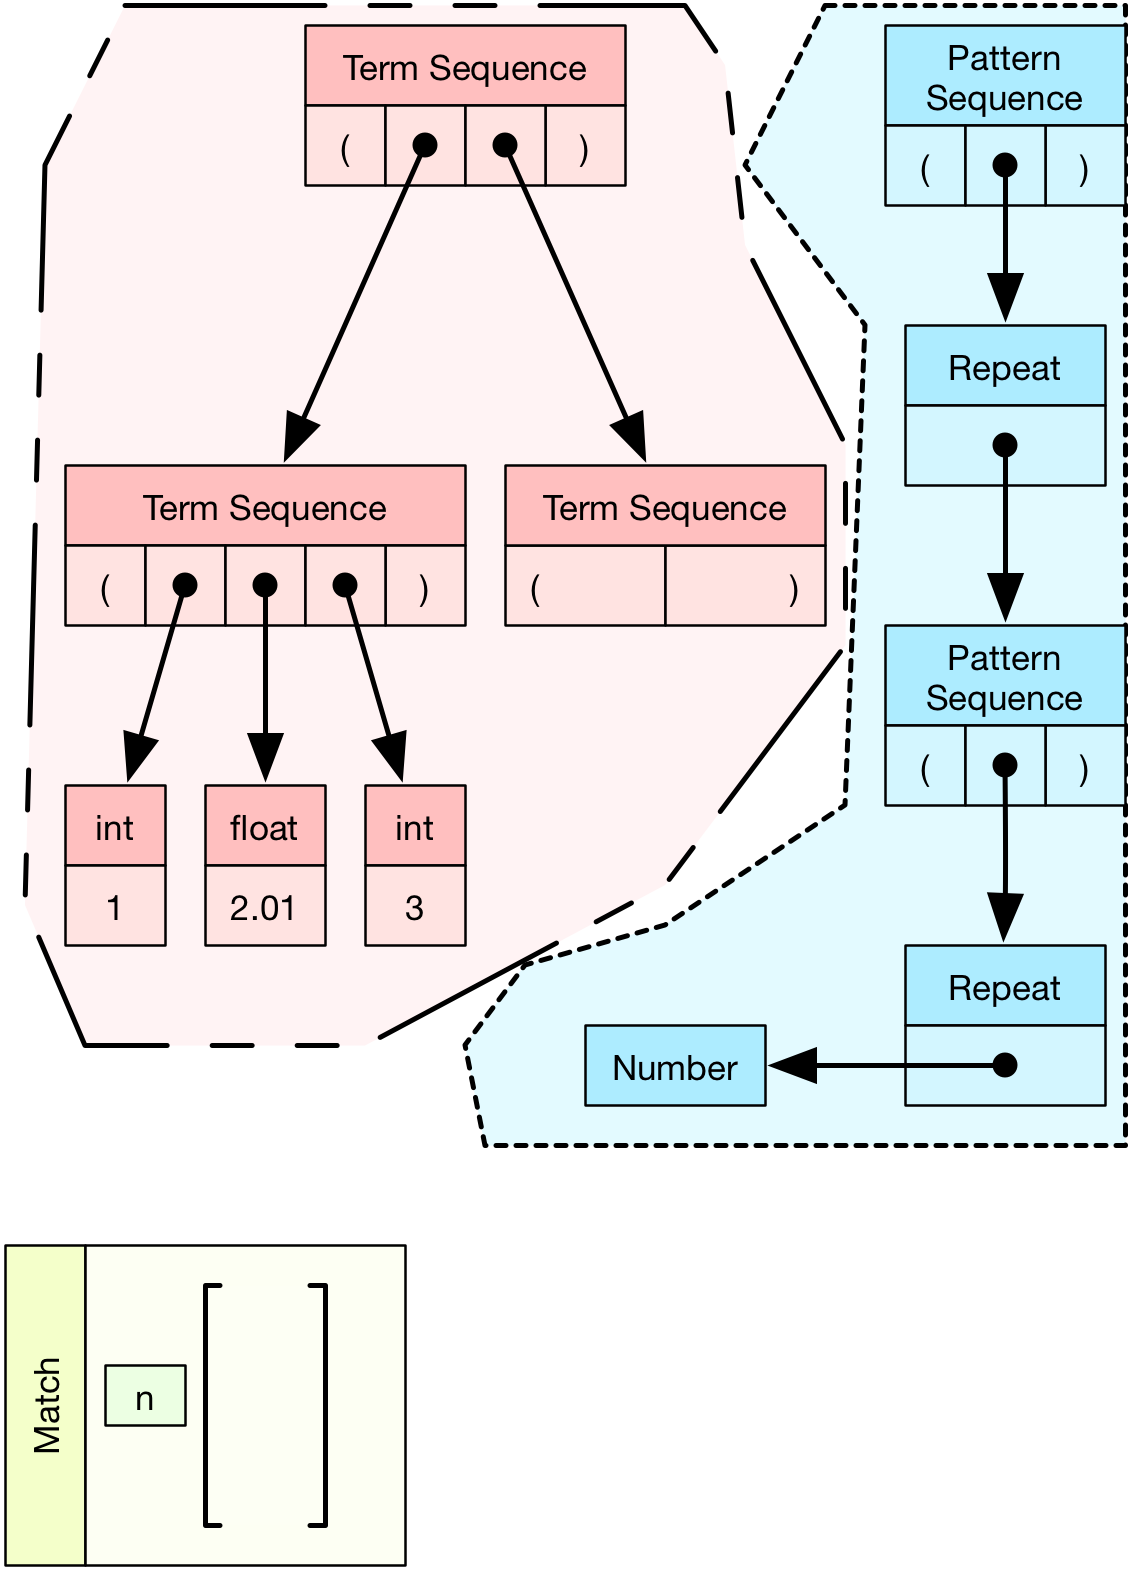
\includegraphics[scale=0.152]{ellipsis-example-fig-a.png}
		}
		\caption{Before matching the pattern.}
		\label{ellipsis-example-fig-a}
	\end{subfigure}
	\begin{subfigure}{0.5\linewidth}
		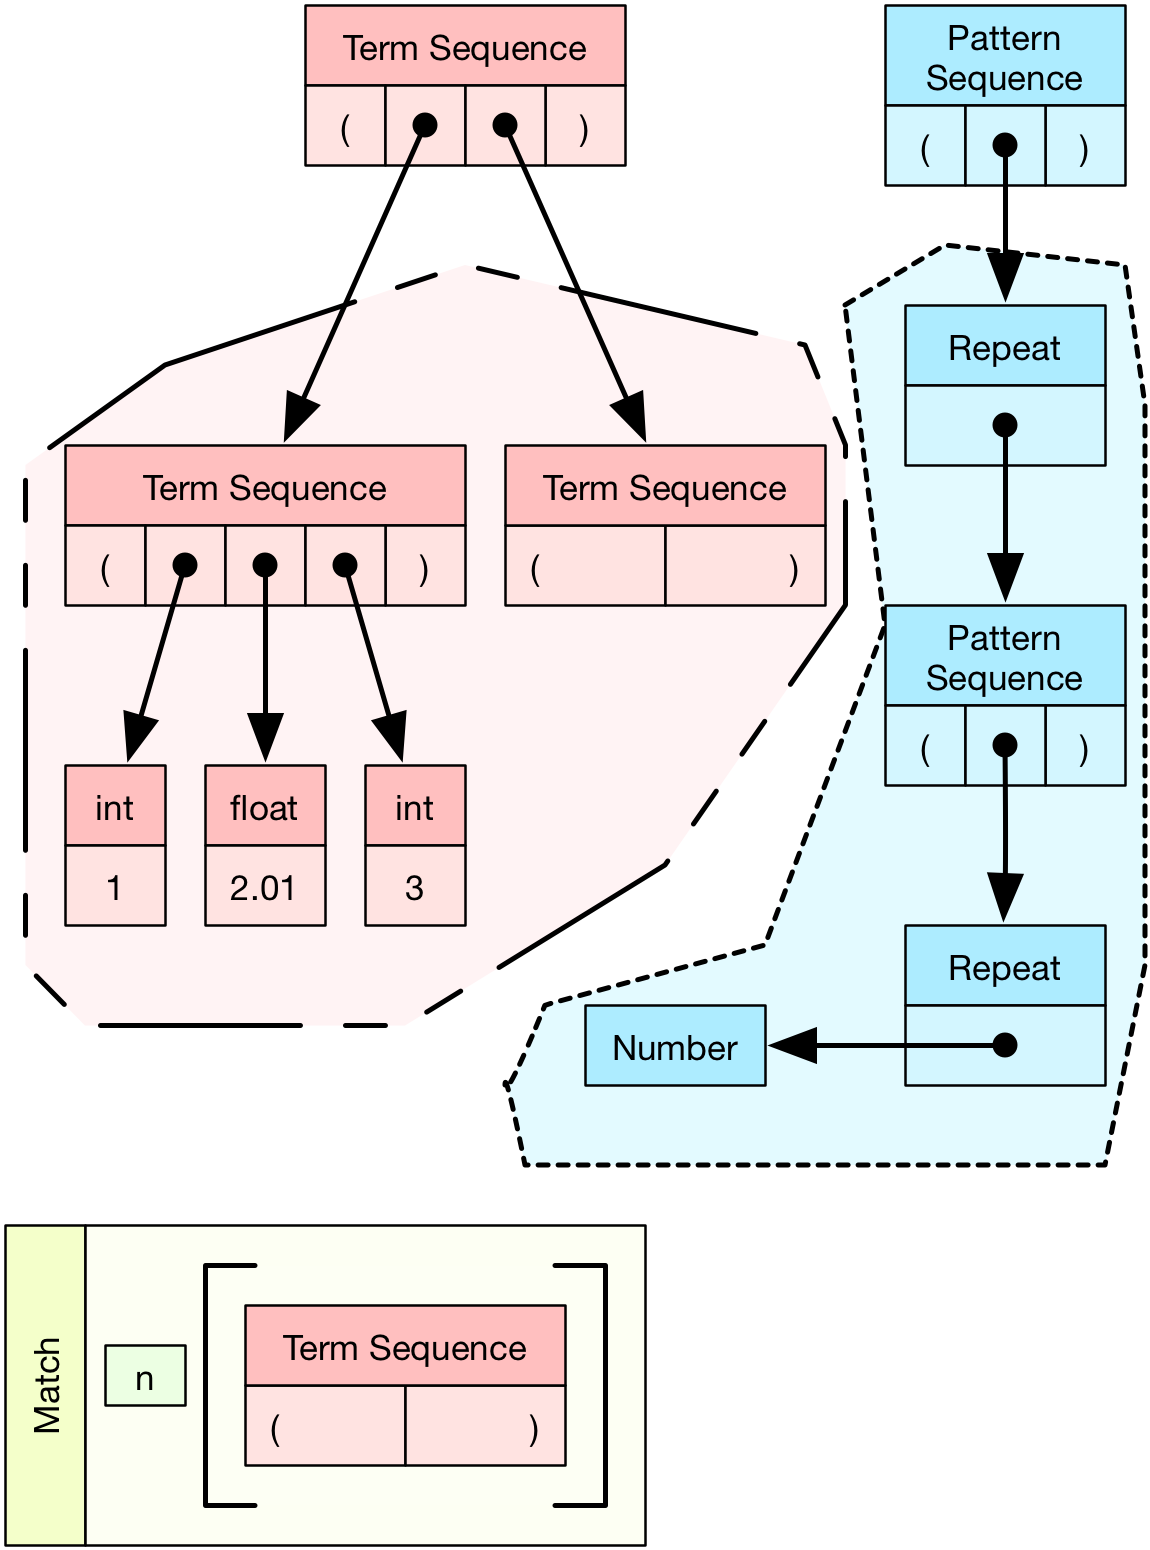
\includegraphics[scale=0.152]{ellipsis-example-fig-b.png}
		\caption{Enter outer ellipsis and \texttt{increasedepth("n")}.}
		\label{ellipsis-example-fig-b}
	\end{subfigure}
}

\fbox{
	\begin{subfigure}{0.5\linewidth}
		\raisebox{19mm}{
			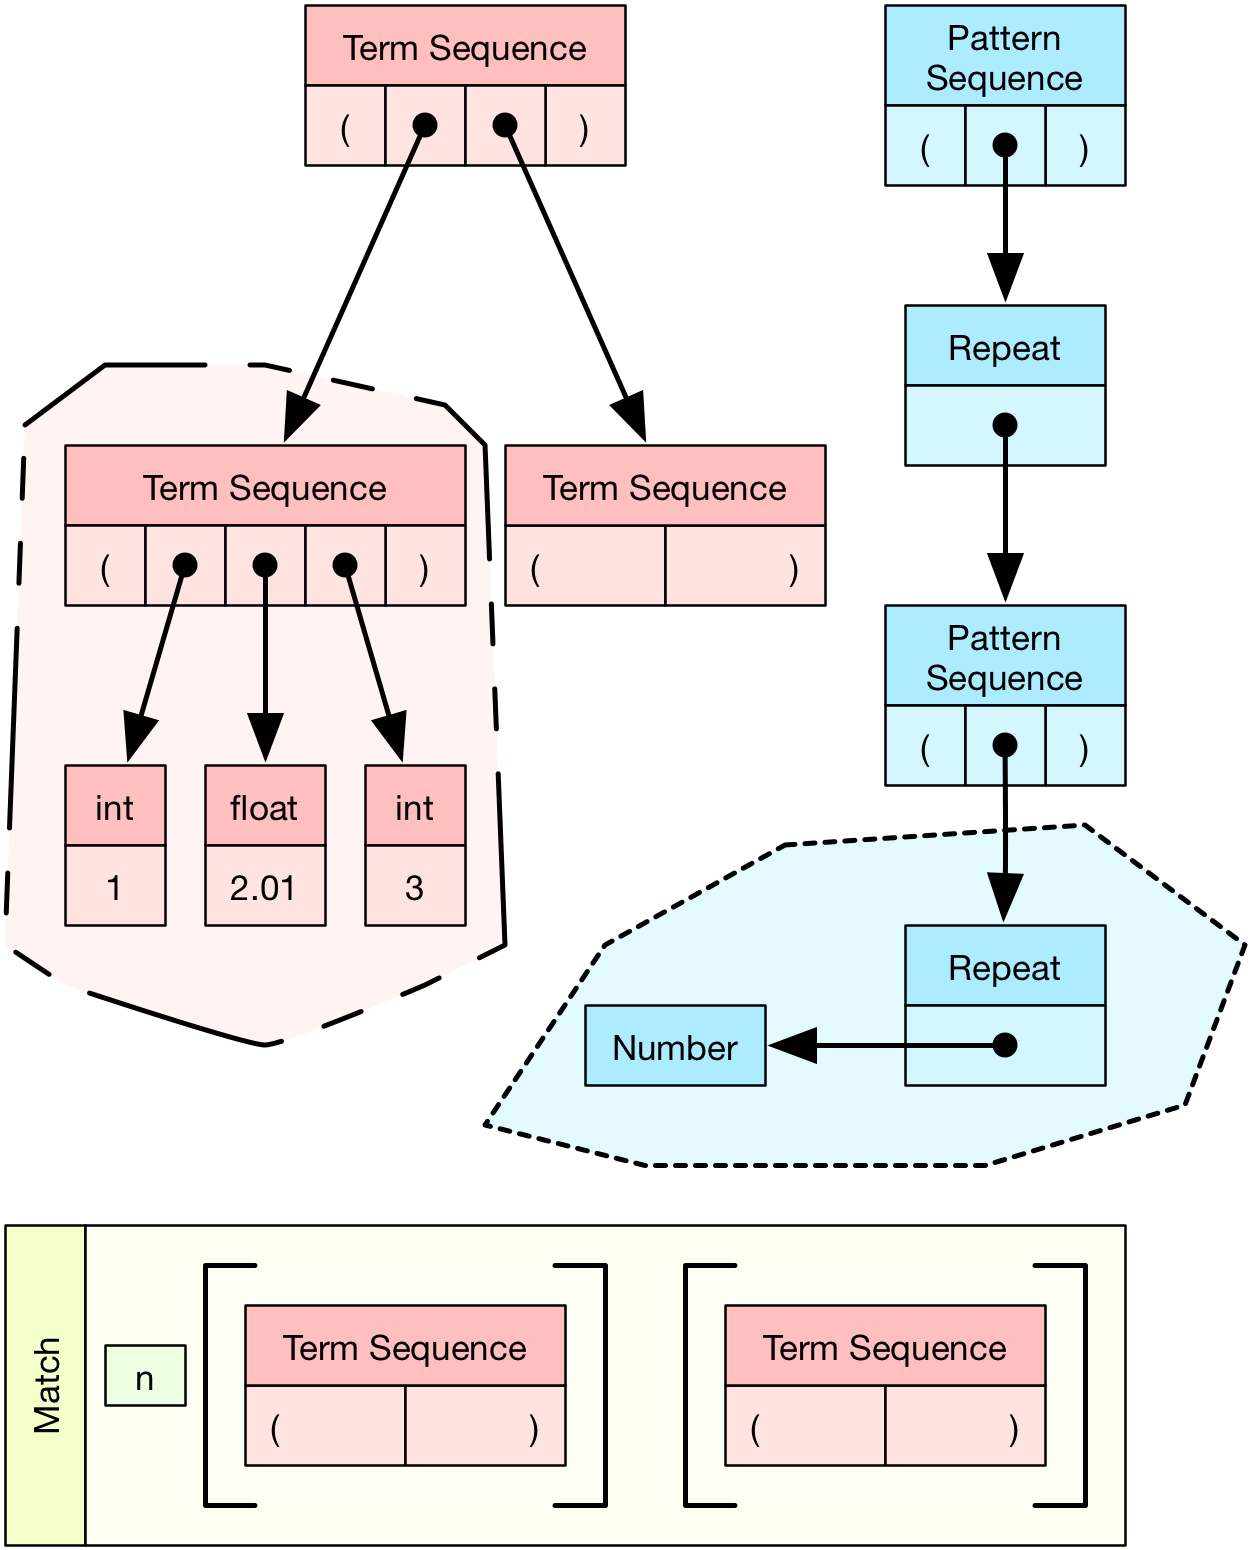
\includegraphics[scale=0.152]{ellipsis-example-fig-c.png}
		}
		\caption{Enter inner ellipsis and \texttt{increasedepth("n")}.}
		\label{ellipsis-example-fig-c}
	\end{subfigure}
	\begin{subfigure}{0.5\linewidth}
		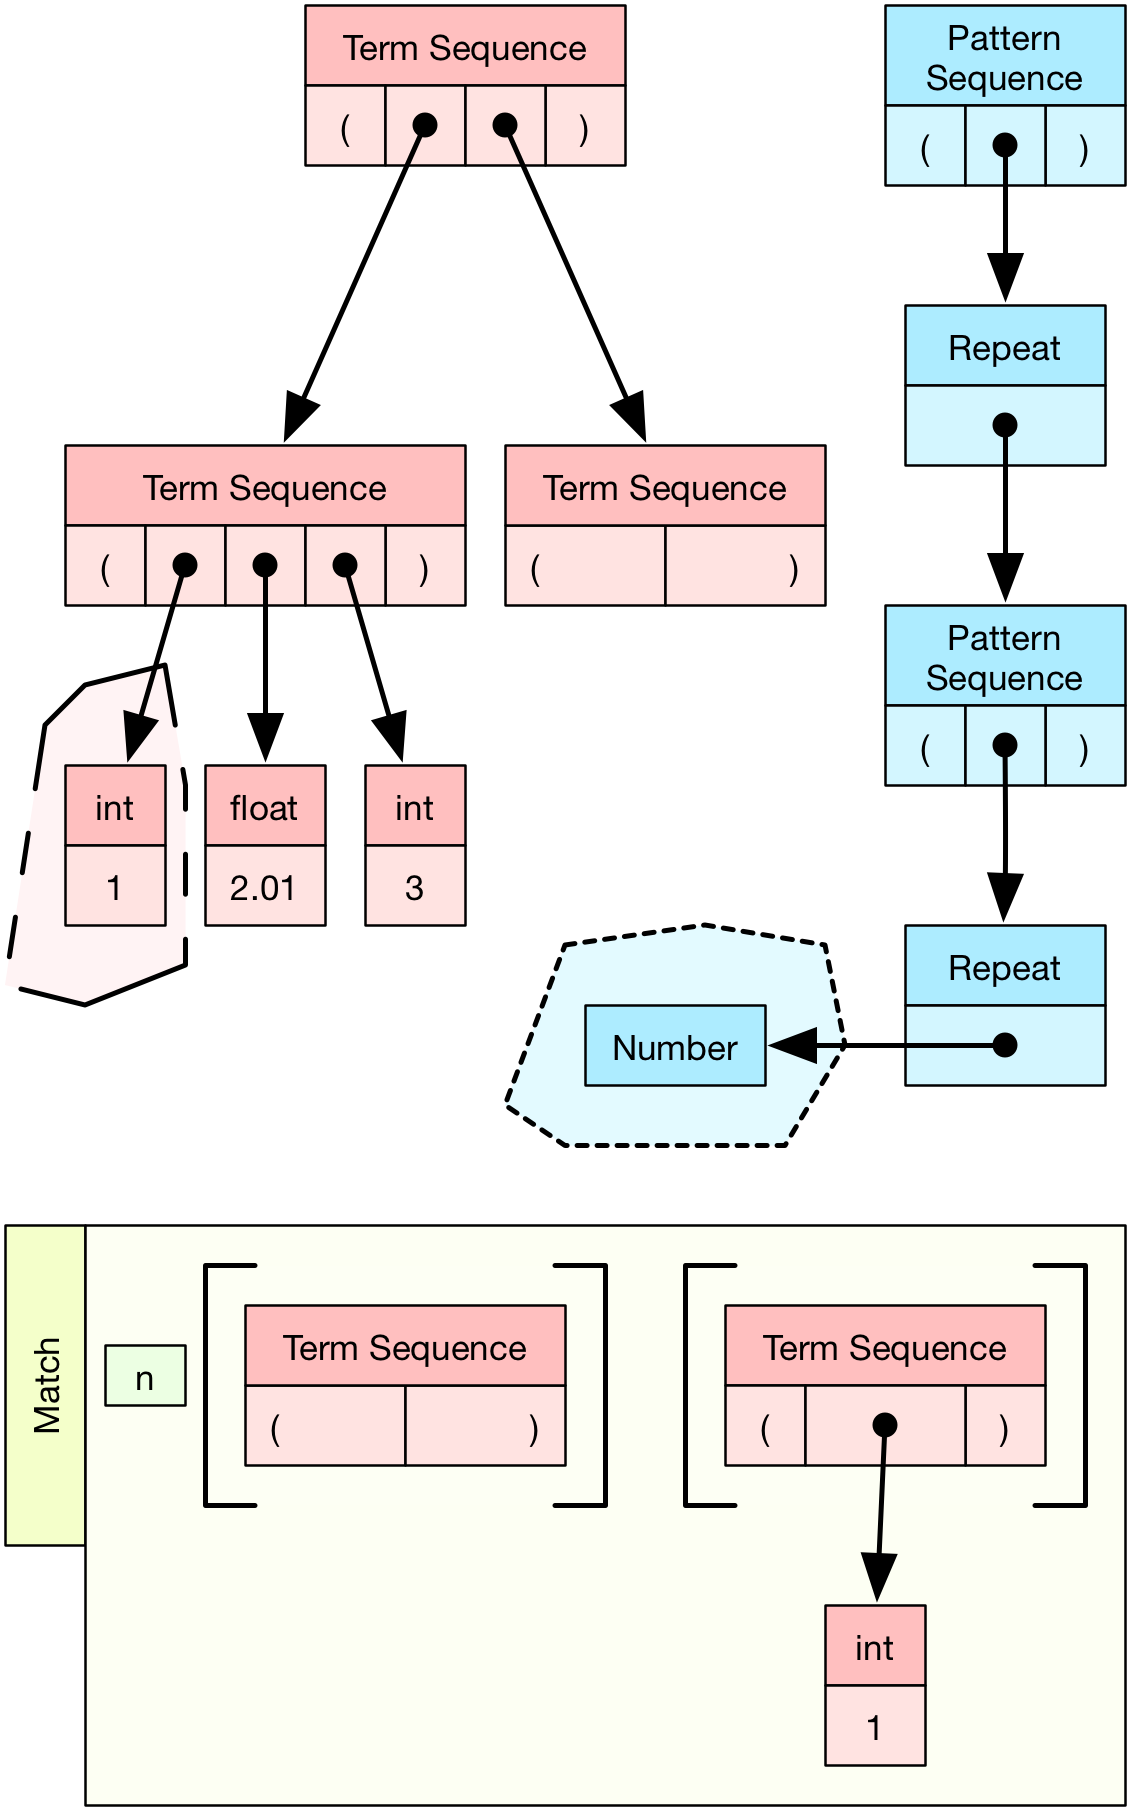
\includegraphics[scale=0.152]{ellipsis-example-fig-d.png}
		\caption{\texttt{addtobinding("n", Integer(1))}}
		\label{ellipsis-example-fig-d}
	\end{subfigure}
}

%\end{adjustwidth}
\end{figure}

\begin{figure}[H]\ContinuedFloat
\fbox{
	\begin{subfigure}{0.5\linewidth}
		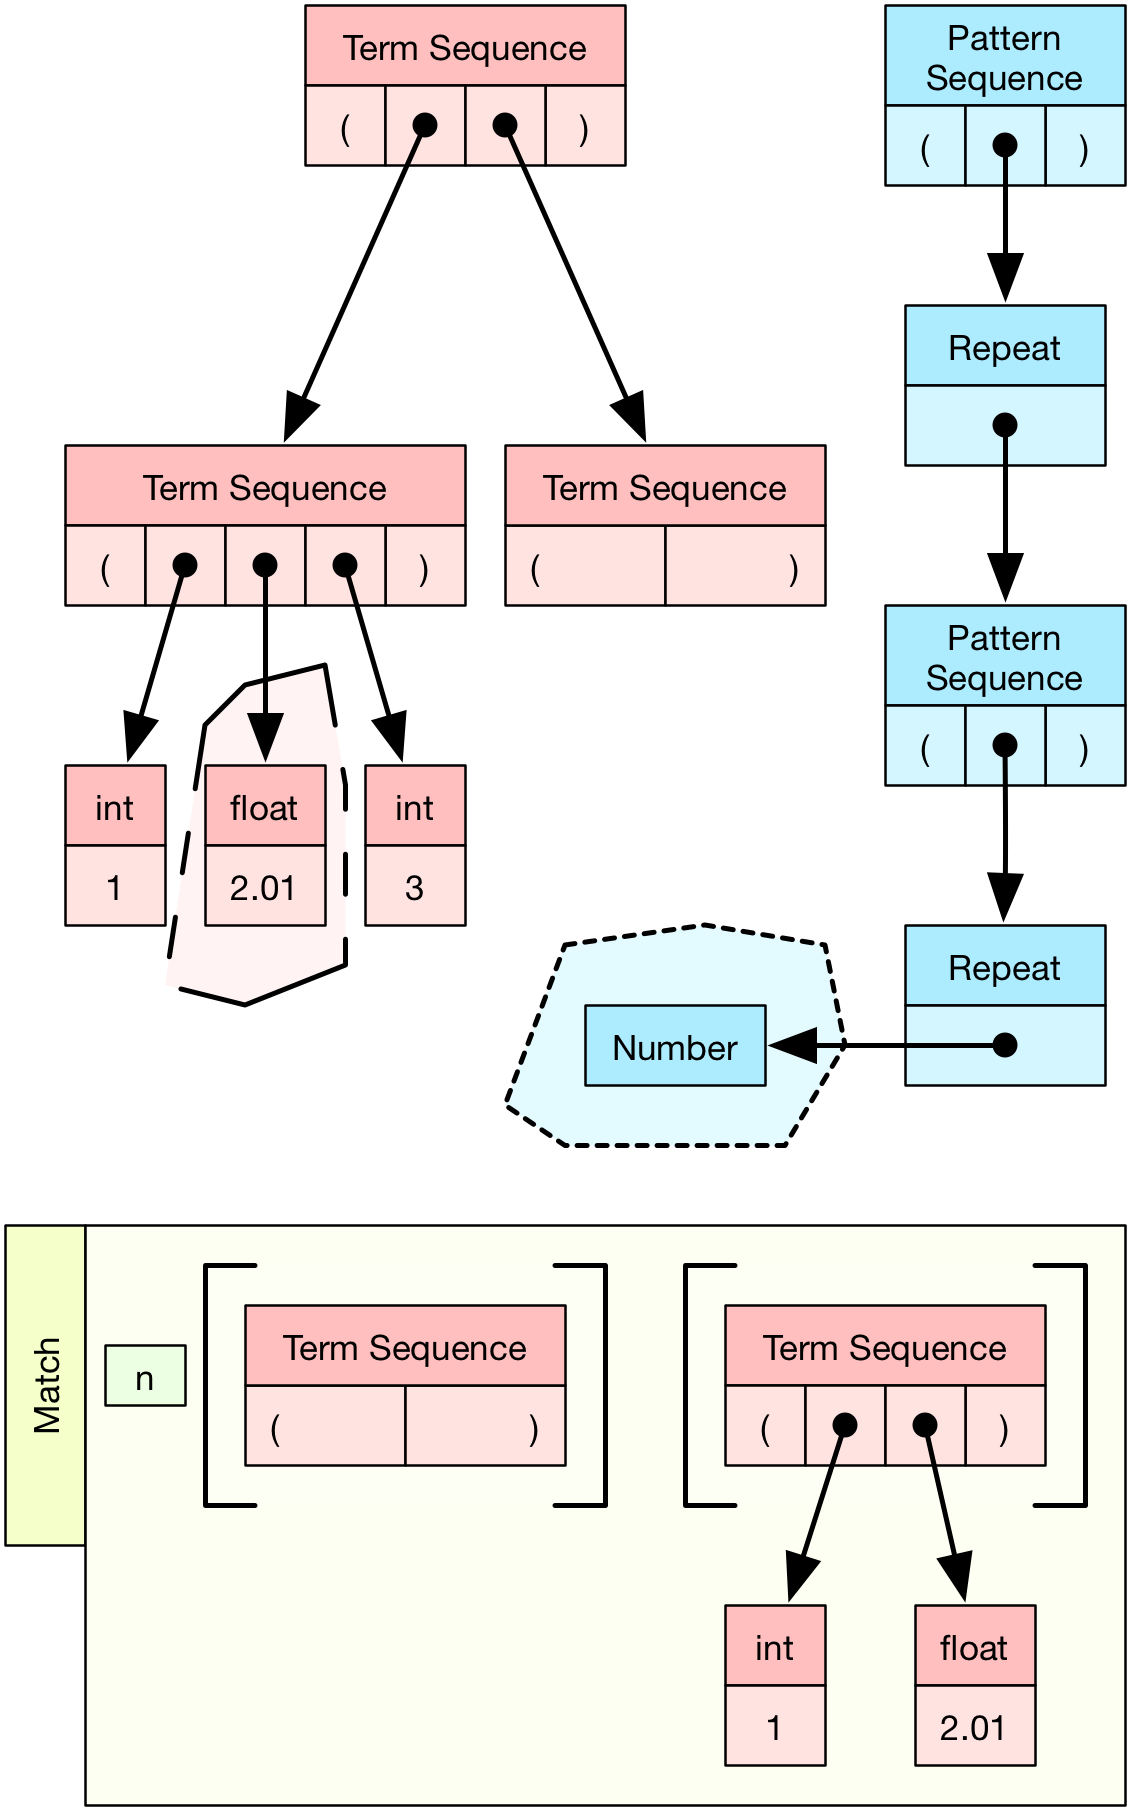
\includegraphics[scale=0.152]{ellipsis-example-fig-e.png}
		\caption{\texttt{addtobinding("n", Float(2.01))}}
		\label{ellipsis-example-fig-e}
	\end{subfigure}
	\begin{subfigure}{0.5\linewidth}
		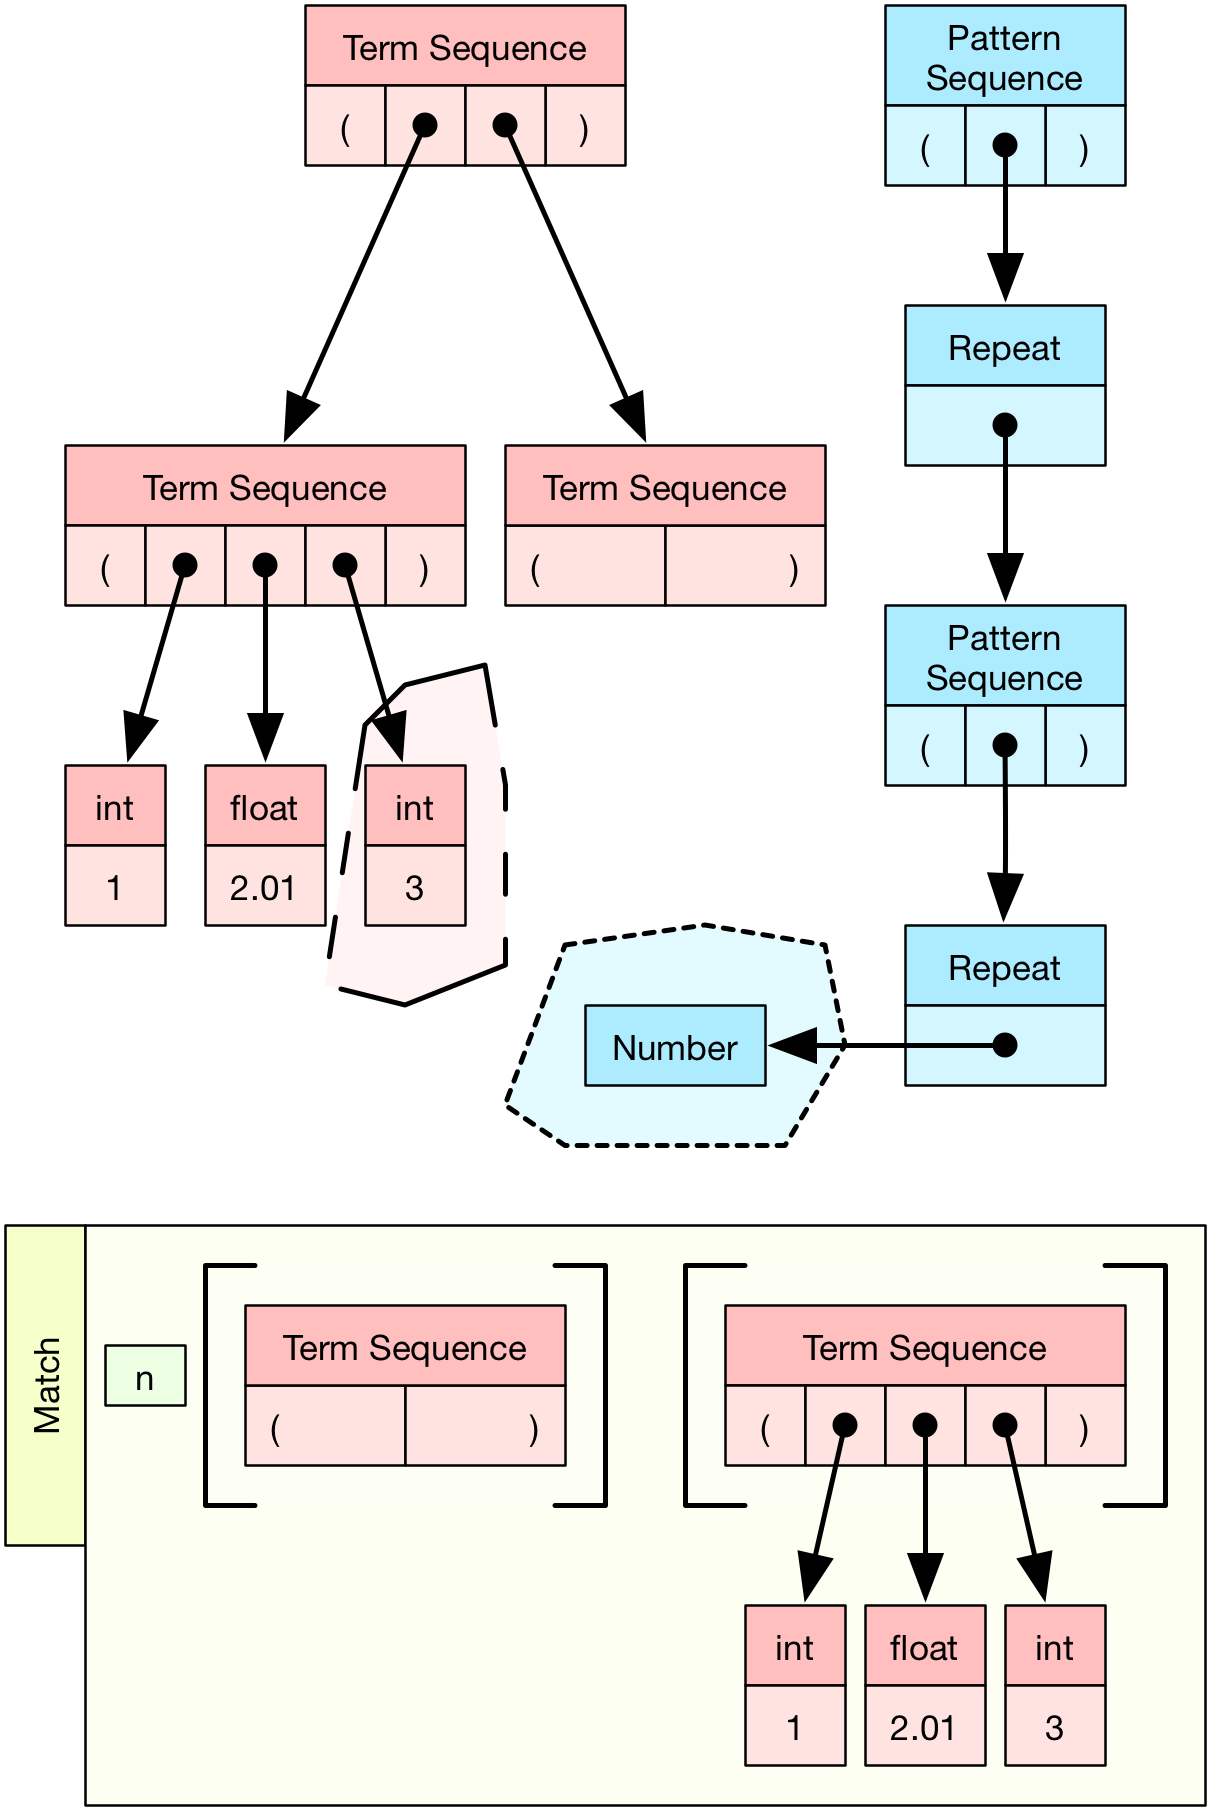
\includegraphics[scale=0.152]{ellipsis-example-fig-f.png}
		\caption{\texttt{addtobinding("n", Integer(3))}}
		\label{ellipsis-example-fig-f}
	\end{subfigure}
}
\fbox{
\begin{subfigure}{0.5\linewidth}
	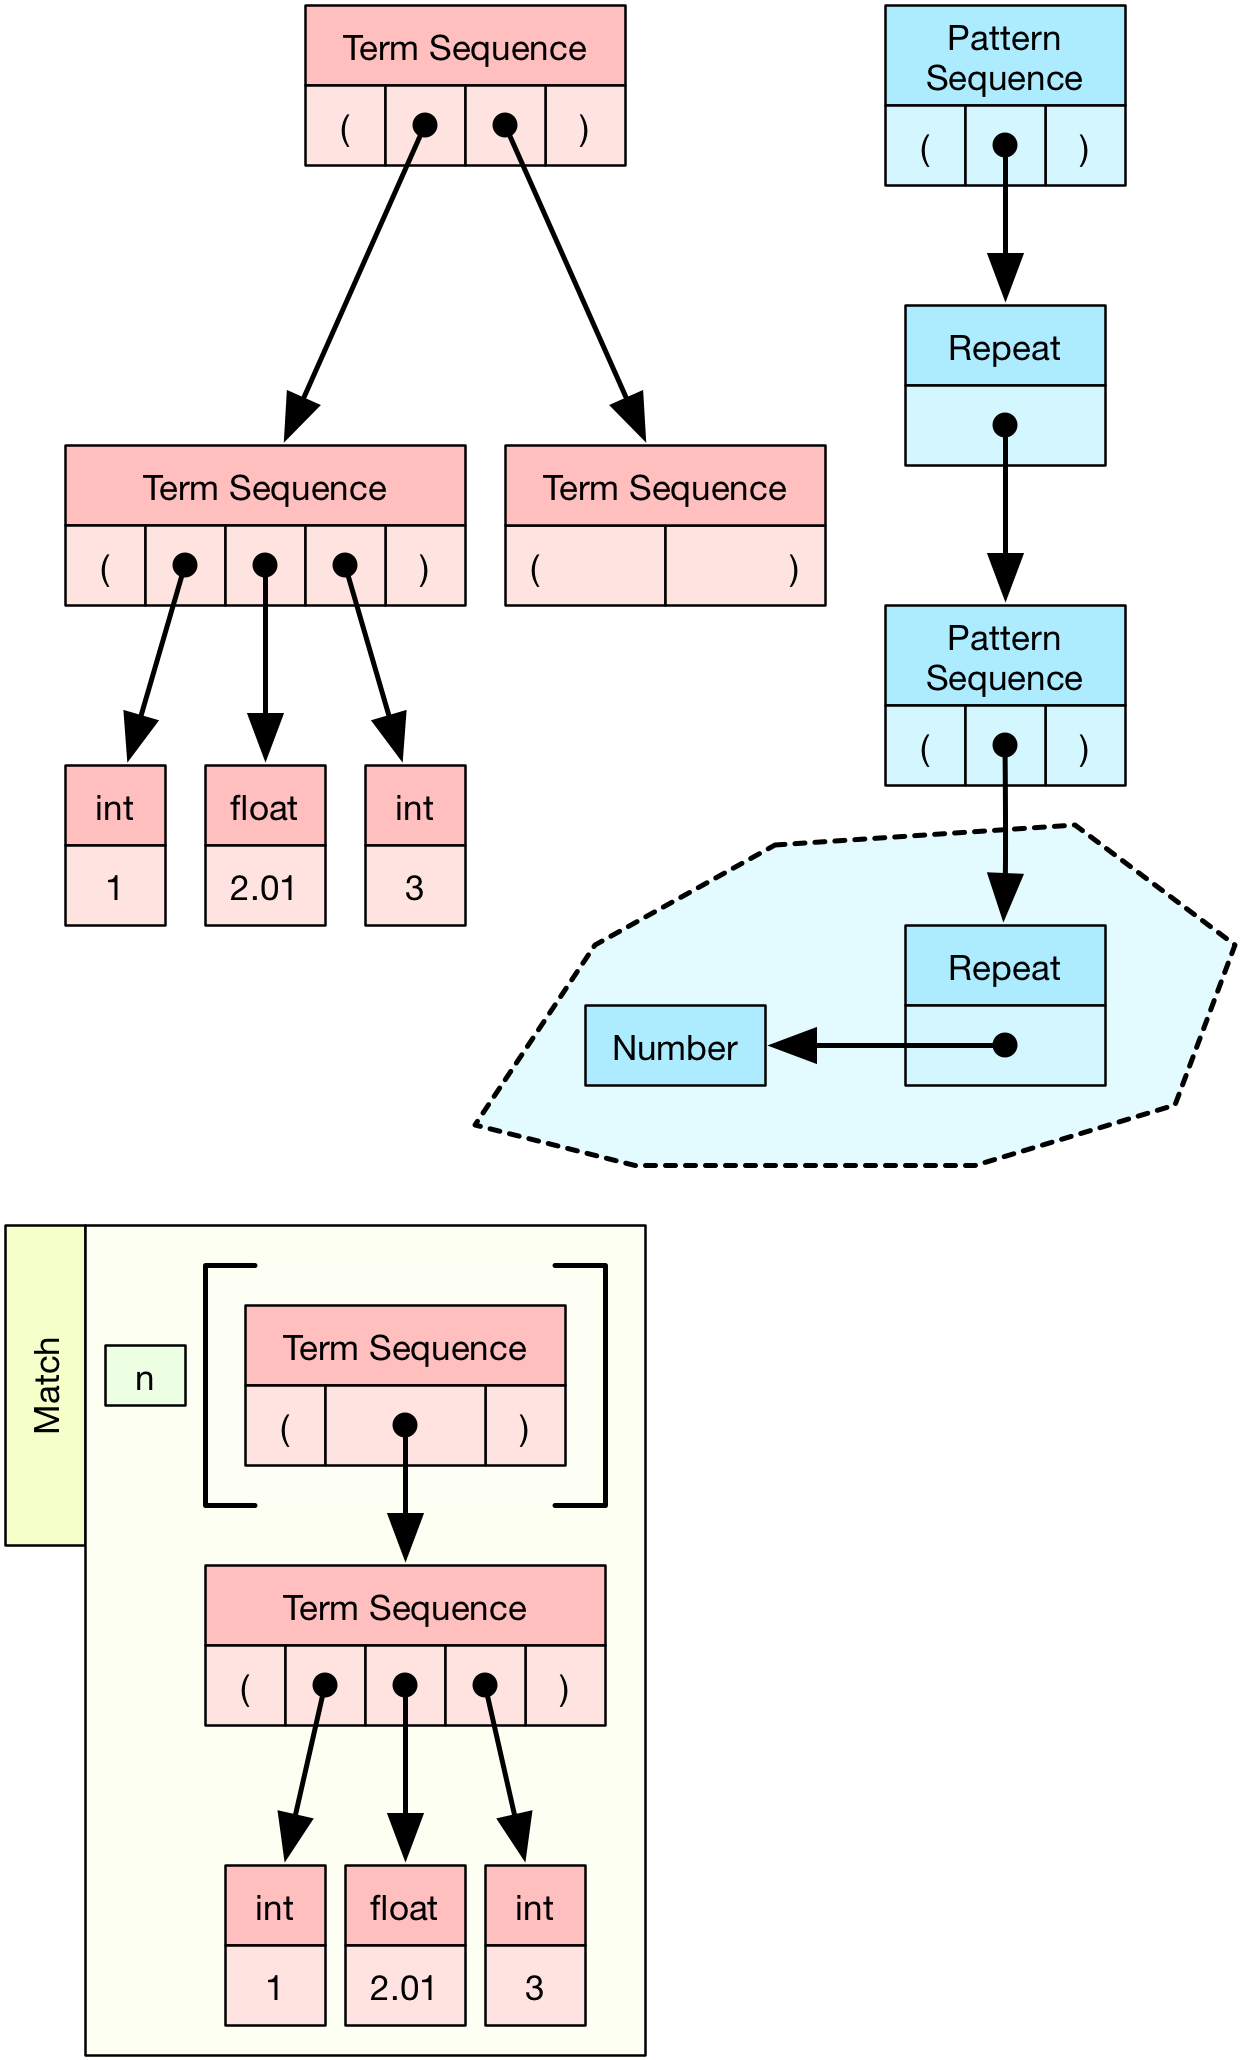
\includegraphics[scale=0.152]{ellipsis-example-fig-g.png}
	\caption{\texttt{decreasedepth("n")} and leave inner ellipsis.}
	\label{ellipsis-example-fig-g}
\end{subfigure}
\begin{subfigure}{0.5\linewidth}
	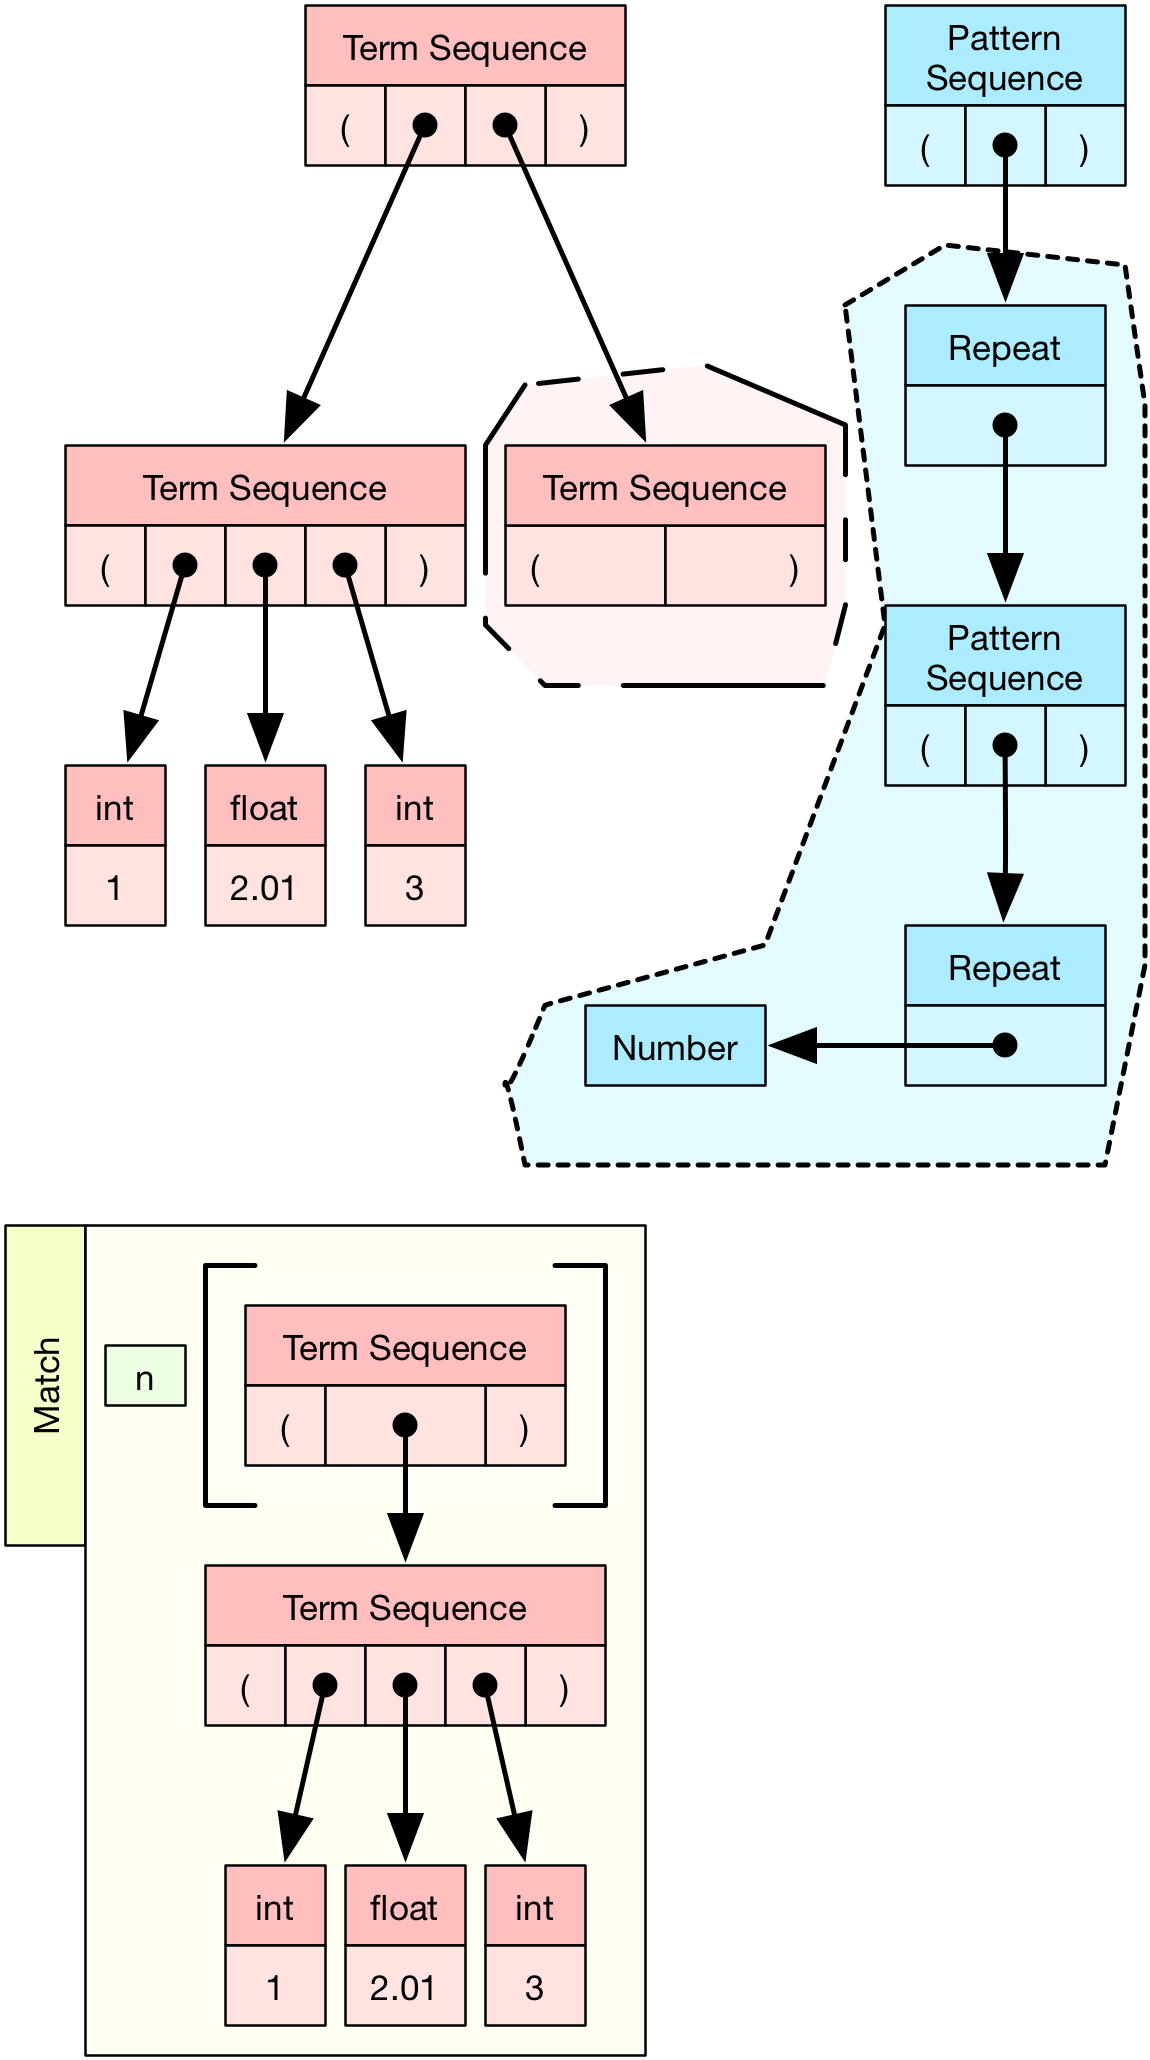
\includegraphics[scale=0.152]{ellipsis-example-fig-h.png}
	\caption{Start processing the next term in the sequence.}
	\label{ellipsis-example-fig-h}
\end{subfigure}
}
\end{figure}
\begin{figure}[H]\ContinuedFloat
\fbox{
	\begin{subfigure}{0.5\linewidth}
		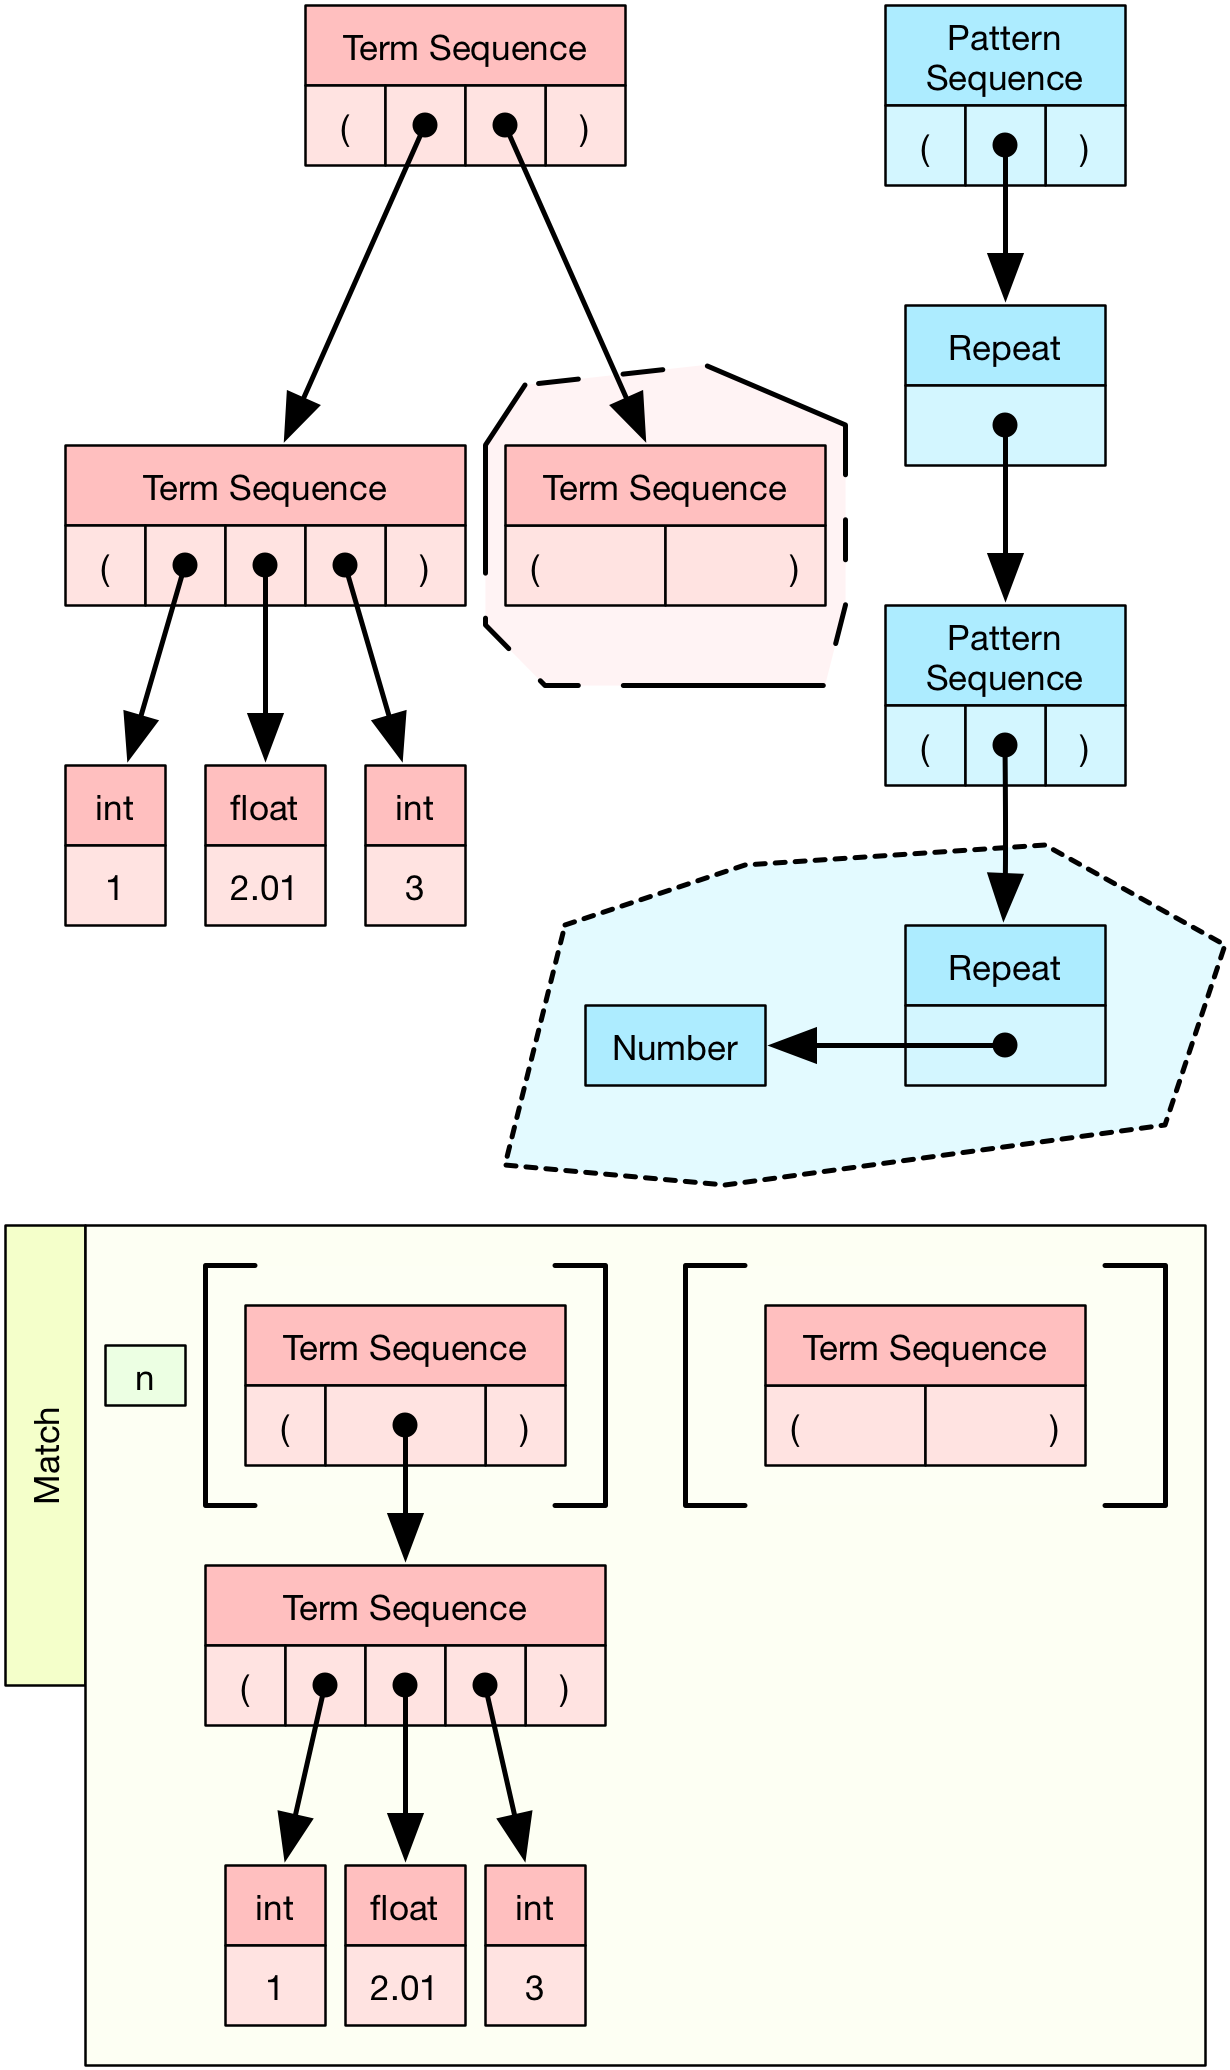
\includegraphics[scale=0.152]{ellipsis-example-fig-i.png}
		\caption{\texttt{increasedepth("n")} after entering inner ellipsis.}
		\label{ellipsis-example-fig-i}
	\end{subfigure}
	\begin{subfigure}{0.5\linewidth}
		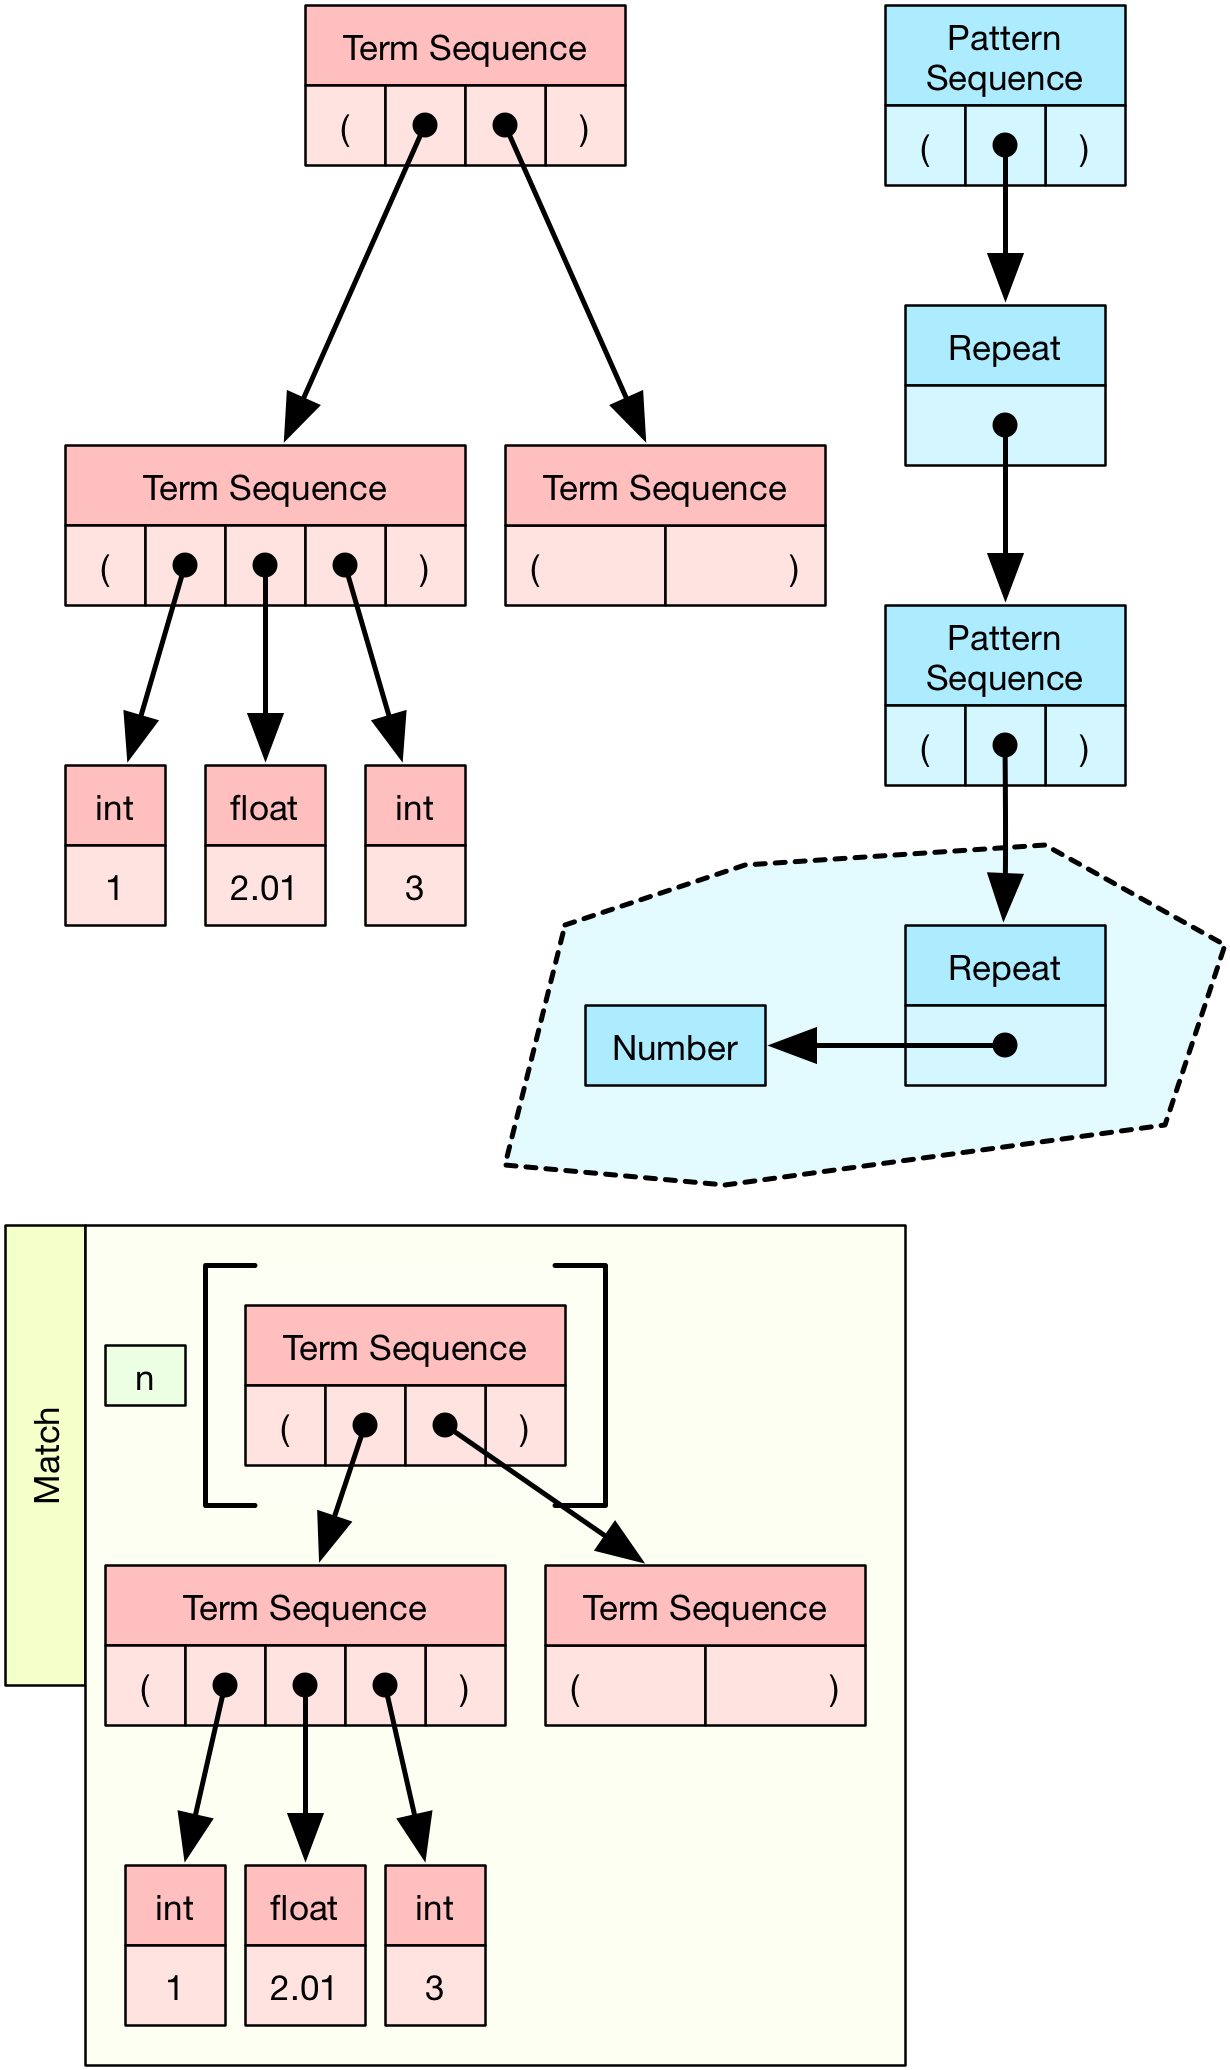
\includegraphics[scale=0.152]{ellipsis-example-fig-j.png}
		\caption{\texttt{decreasedepth("n")} and leave inner ellipsis.}
		\label{ellipsis-example-fig-j}
	\end{subfigure}
}

\fbox{
	\begin{subfigure}{0.5\linewidth}
		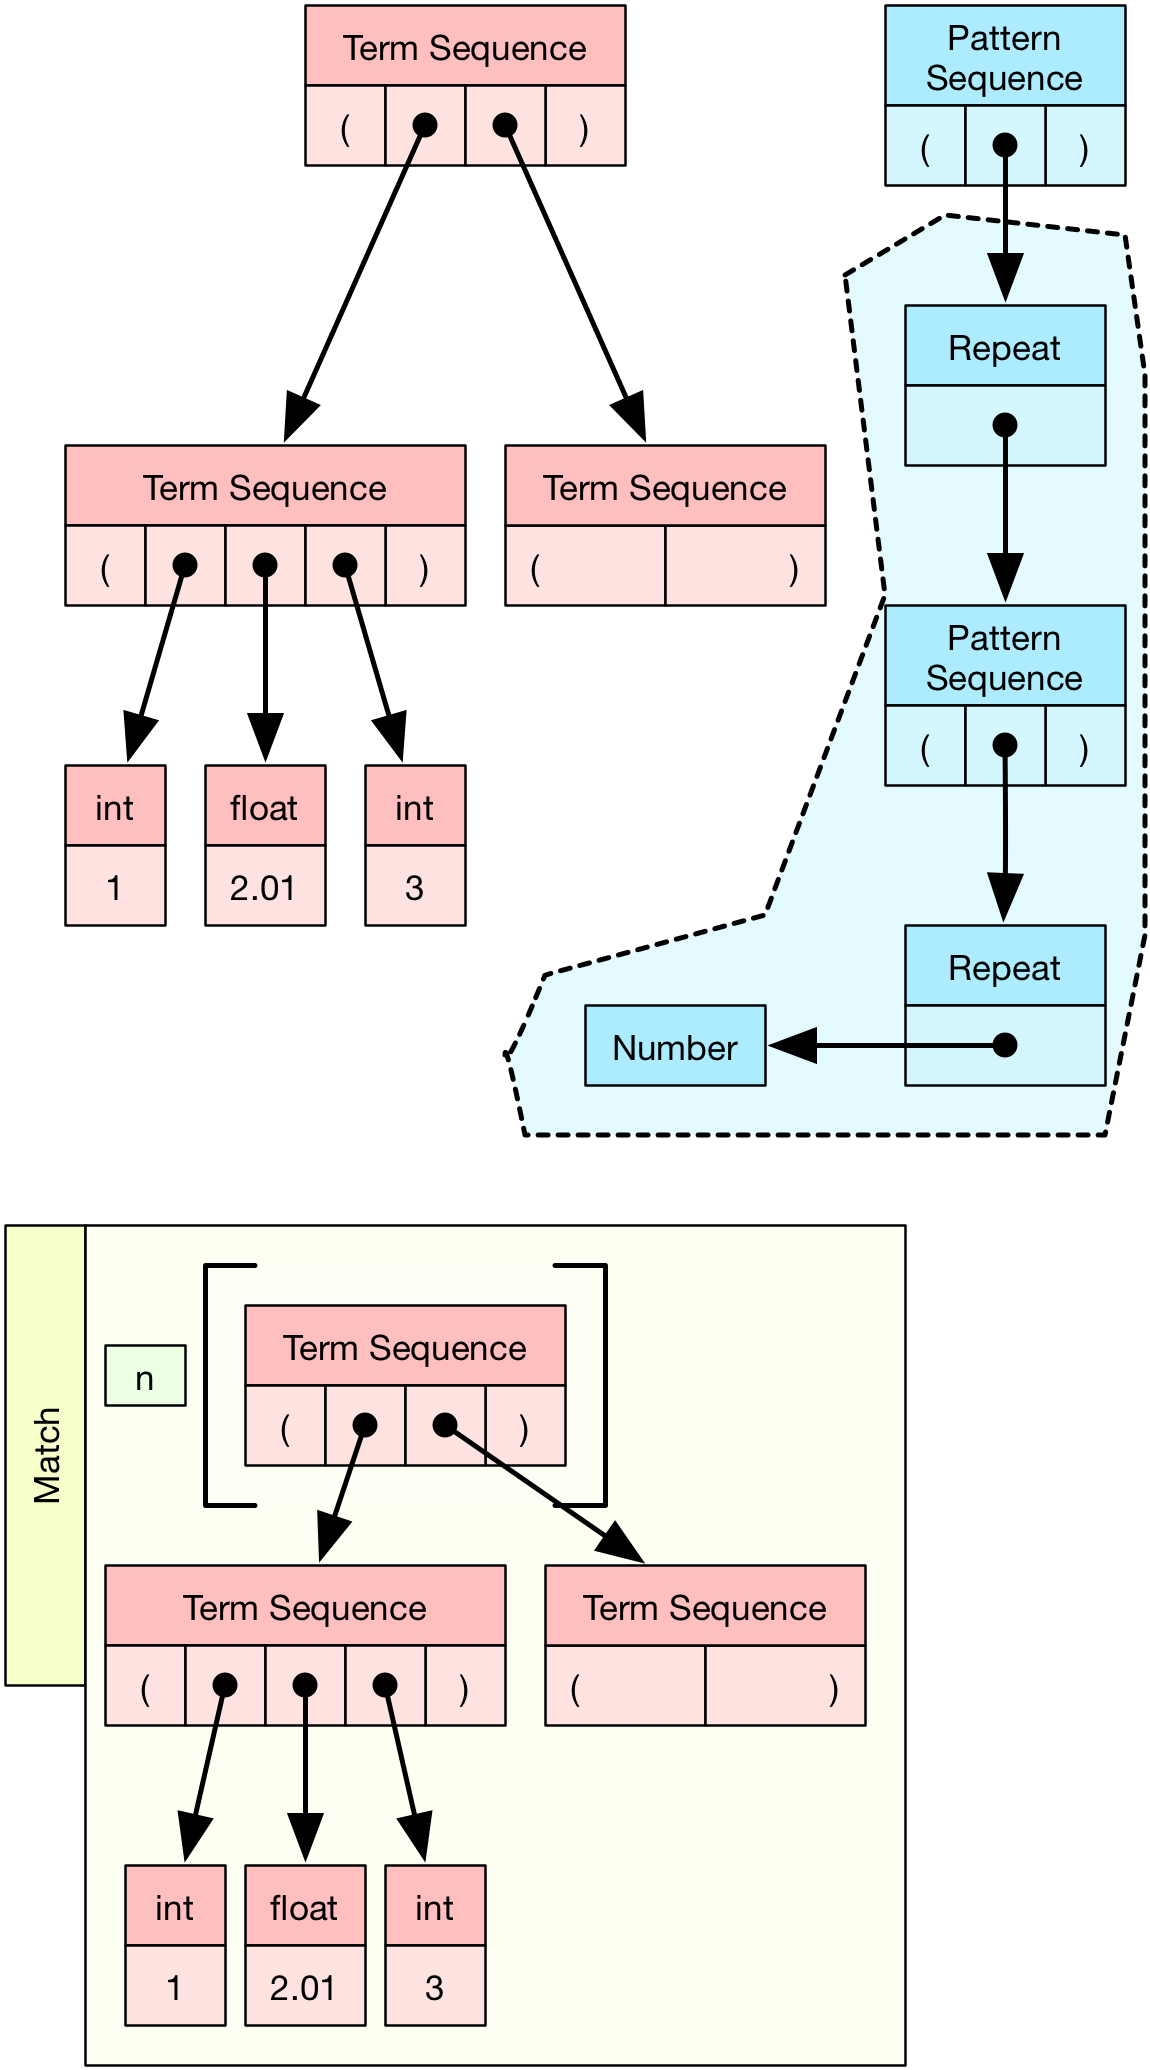
\includegraphics[scale=0.152]{ellipsis-example-fig-k.png}
		\caption{\texttt{decreasedepth("n") and leave outer ellipsis}.}
		\label{ellipsis-example-fig-k}
	\end{subfigure}
}
\end{figure}



Of course, in ellipsis matching algorithm one may notice this example does not demonstrate all possible matches, but only lifetime of the only surviving match. In fact, after matching (1 2.01 3) against ( n ...) the following matches would be produced by ellipsis:

n =         0 3
n = ((1))   1 3
n = ((1 2)) 2 3
n = ((1 2 3)) 3 3
But the only one surviving is the one that has match all the terms. 

TODO 
